\documentclass[runningheads]{llncs}
\usepackage{graphicx}
\usepackage{subfig}
\usepackage[font = small, labelfont=bf]{caption}
\usepackage{verbatim}
\usepackage{amsmath}
% If you use the hyperref package, please uncomment the following line
% to display URLs in blue roman font according to Springer's eBook style:
\usepackage{hyperref}
\usepackage{xcolor}
\usepackage{commath}            %For norm command
\renewcommand\UrlFont{\color{blue}\rmfamily}

\begin{document}

\title{Vector Calculation of Moment Arms of Human Muscles about Monoarticular and Biarticular Joints}
\titlerunning{Vector Calculation of Moment Arms for Muscles}

%\author{Connor Morrow\orcidID{000-0001-5468-9032}, Alexander Hunt\orcidID{0000-0002-3820-4821}}
\author{Connor Morrow\orcidID{000-0001-5468-9032}}
\authorrunning{C. Morrow}

\institute{Department of Mechanical and Materials Engineering, Portland State University, Portland, OR 97207, USA\\
\email{comorrow@pdx.edu}}

\maketitle              % typeset the header of the contribution
\begin{abstract}
This paper documents a methodology for calculating the moment arms that human muscles create when they contract and actuate a joint they pass over. The method for calculating the moment arm requires knowing the vectorized direction of the muscle in the coordinate frame of the joint. This process is then expanded to calculate how the moment arm changes as the joint it passes over moves to different positions. Moment arm profiles for selected muscles of the hip and knee joint are presented. The calculations for the muscle moment arms is also extended from monoarticular muscles to biarticular muscles. The process developed here provides a basis for calculating the maximum amount of torque that muscles are able to generate about joints, which will provide a comparison for the amount of torque that braided pneumatic actuators can create about the joints of a bipedal humanoid robot. 

\keywords{Biomechanics \and Moment Arm \and Monoarticular Muscles \and Biarticular Muscles \and OpenSim \and Matlab}
\end{abstract}

\section{Introduction}
Hypotheses: By reducing muscles to either a single or group of straight line actuators, the moment are can be calculated about a joint and produce a torque result that is close to the actual torque that a human can produce with those same muscles.

In order to actuate robots in a biomimetic manner, it becomes of paramount importance to understand how muscles actuate skeletal structures. Many organisms use muscles in order to drive actuation. A muscle attaches to a bone, passes over one or more joints, and inserts itself into another bone. When the muscle contracts, it generates a tensile force from the inserted bone to the original attachment bone along the length of the muscles. This contractions generates a torque about the joint, which causes rotation. 

Creating a way of calculating the moment arm is a good focus of research as it helps us emulate this contraction to joint rotation on robotics. 

Presented here is a way of calculating the moment arm of a muscle, when it is assumed to be a series of straight line actuators. 


\section{Methods}
\label{methods}
The analysis presented here is based off the physiology that is displayed in the OpenSim model gait2952. OpenSim is a platform in which researchers can explore the human musculoskeletal structure. Gait2952 is a human model of the lower torso and legs, and includes 92 actuators that represent 72 human muscles. These actuators are displayed as straight lines that start at an origin point and end at an insertion point, with many actuators including via or wrapping points in between the origin and insertion which capture the changing direction of muscles in the human body without curving the muscles themselves. 


\subsection{Vector Analysis of Moment Arms}
The calculation of a moment arm of a muscle that passes over a joint was done by using vector analysis and transformation matrices. The transformation matrices will be discussed in the next section. In this section, we will explore a vector algorithm that will be able to calculate the length and direction of a moment arm in the coordinate frame of a joint. 

A moment arm is the vector that originates at the origin of a reference frame. When the moment arm is crossed with a force vector, a torque is produced. If we know the spatial coordinates of the reference frame as well as two points that define the line of action of the force vector, we can derive the moment arm to that vector. 

\subsection{Transformation Matrices}
Muscles generate torque by contracting about a joint. Because a muscle has complicated geometry, calculating the torque about a joint can be simplified by creating one or more linear approximations for the muscle geometry as it passes over joints. OpenSim provides the linear approximations of the muscles by listing origin points, attachment points, and wrapping or via points. Each of these points are given coordinates within a joint reference frame and are connected to one another with straight lines.

Because muscles have multiple points along their geometric path that reside in two or more reference frames, it is important to determine the orientation and spacial distance between each of these reference frames in order to accurately calculate the moment arm. With this in mind, each joint reference frame is prescribed a transformation matrix that relates it to it's parent reference frame, or the reference frame of the joint that precedes it in the path of the muscle.

In order to construct a transformation matrix, we first need to calculate the rotation matrix of a frame. A rotation matrix requires knowledge about how the axes of a coordinate frame has rotated away from it origin or home position. The home position of the OpenSim model has all of the coordinate frames in the same orientation, meaning there is no rotation along any of the axes. The axes all list the x axis as pointing along the anterior direction away from the model within the sagital plane and parallel to the ground. The y axis points in the superior direction, within the sagittal plane, orthogonal to the ground. The z axis points laterally along the horizontal plane, orthogonal to the x and y axis, and parallel to the ground.

%Insert picture of two reference frames, in the same orientation. Maybe two pictures side by side from different angles

When a muscle contracts, it actuates the joint it crosses over, causing the coordinate frame, whose origin is at the center of rotation of a joint, to rotate. This rotation can be quantified with three Euler angles. $/Theta$ defines rotation about the x axis, $\psi$ defines rotation about the y axis, and $\gamma$ defines rotation about the z axis. Using these angles we can construct three rotation matrices which will define the rotation of the coordinate from from it's home position.

\begin{align}
    R_z &= \begin{bmatrix}
                cos\theta && -sin\theta && 0\\
                sin\theta && cos\theta && 0\\
                0 && 0 && 1\\
            \end{bmatrix}\\
    R_y &= \begin{bmatrix}
                cos\phi && 0 && -sin\phi\\
                0 && 1 && 0 && r_y\\
                sin\phi && 0 && cos\phi\\
            \end{bmatrix}\\
    R_x &= \begin{bmatrix}
                1 && 0 && 0 && r_x\\
                0 && cos\gamma && -sin\gamma\\
                0 && sin\gamma && cos\gamma\\
            \end{bmatrix}
\end{align}

With these three rotation matrices, one single rotation matrix can be constructed to make calculations simpler and more concise. 

\begin{align}
    R = R_z * R_y * R_x
\end{align}

Having one rotation matrix allows the creation of a transformation matrix. This transformation matrix defines the translated distance from one coordinate frame to another, while also capturing the relative rotation between the two. For the purposes of the moment arm calculations, the first coordinate frame is assumed to always remain in the home position, while the muscle actuation will cause rotation in the second or third coordinate frame. That means only the rotation matrix for coordinate frames after the first one is required. The distance between coordinate frames can be written in vector form.

\begin{equation}
    \Vec{p} = [x_{2/1} \quad  y_{2/1}  \quad z_{2/1}]
\end{equation}

The subscripts here mean the distance along that axis from coordinate frame one to coordinate frame two. With the vector distances, the transformation matrix can be constructed by attaching the transposed vector p to the rotation matrix and creating a fourth row which contains 0 for the first three columns and a 1 in the last column.

\begin{equation}
    T = \begin{bmatrix}
            R_{11} && R_{12} && R_{13} && p_1\\
            R_{21} && R_{22} && R_{23} && p_2\\
            R_{31} && R_{32} && R_{33} && p_3\\
            0 && 0 && 0 && 1
        \end{bmatrix}
\end{equation}

In order to bring a muscle point into the coordinate reference frame after the one that it is located in, the distance vector describing that point, $\vec{s}_n$, first needs to appended with a 1 in the fourth position of the vector.

\begin{equation}
    \Vec{s}_n^{\prime} = [\Vec{s}_n \quad 1]\\
\end{equation}

Then, we can premultiply that vector by the transformation matrix. Once we remove the fourth element of this new vector and transpose it, then we have the row vector that describes the location of that point in the new reference frame.

\begin{equation}
    \Vec{s}_{n+1}' = T*\Vec{s}_n;\\
\end{equation}
\begin{equation}
    \Vec{s}_{n+1} = [s_1 \quad s_2 \quad s_3]
\end{equation}

\subsection{Moment Arm Calculation}
With the points that define a line of the muscle that passes over a joint all within the same coordinate frame of the joint, we can begin to calculate the moment arm. The moment arm will be the distance vector starting from the joint coordinate frame to the muscle line and orthogonal to the direction of the muscle.

To calculate the moment arm, the first step is to define the vector that makes up the direction and magnitude of the muscle segment length. This is done by moving the first point that defines the muscle segment, located in the first frame, into the second frame. In order to find the vector in the second frame, the transformation matrix that defines the second frame relative to the first frame is divided by an identity matrix. Then the vector is multiplied by this result.

\begin{equation}
    \Vec{s}_{1/2} = \dfrac{T}{I} * \Vec{s}_1
\end{equation}

The vector that defines the muscle segment can easily be obtained from this by subtracting $\Vec{s}_2$ from $\Vec{s}_{1/2}$.

\begin{equation}
    \Vec{m} = \Vec{s}_{1/2} - \Vec{s}_2
\end{equation}

The unit vector that defines the muscle vector is calculated by dividing the muscle vector by it's magnitude.

\begin{equation}
    \hat{u} = \dfrac{\Vec{m}}{|\Vec{m}|}
\end{equation}

Now that the unit vector of the muscle segment is defined, we can calculate the moment arm. By taking the dot product of $\hat{u}$ and $\Vec{s}_2$ we are able to find the distance along the muscle vector in which it is orthogonal to the coordinate frame. Then by multiplying this magnitude by $\hat{u}$, we create a new vector, which begins at the tip of $\Vec{s}_2$ and points to the location along the muscle segment that is orthoganal to the origin of the coordinate frame.

\begin{equation}
    \Vec{w} = \hat{u}(\hat{u} \cdot \vec{s}_2)
\end{equation}

The moment arm can then be calculated by subtracting $\Vec{s}_2$ by $\Vec{w}$.

\begin{equation}
    \Vec{mA} = \Vec{s}_2 - \Vec{w}
\end{equation}

Combining all of these steps gives us the full equation.

\begin{equation}
    \Vec{mA} = \Vec{s}_2 - \dfrac{\dfrac{T}{I}\Vec{s}_1 - \Vec{s}_2}{\norm{\dfrac{T}{I}\Vec{s}_1 - \Vec{s}_2}}\left(\dfrac{\dfrac{T}{I}\Vec{s}_1 - \Vec{s}_2}{\norm{\dfrac{T}{I}\Vec{s}_1 - \Vec{s}_2}} \cdot \Vec{s}_2\right)
    \label{mA}
\end{equation} 

\subsection{Moment Arm Calculation for Monoarticulate Muscles}

A monoarticulate muscle is a muscle that passes over one joint. This is the simplest type of muscle in which to calculate the moment arm and we are able to use equation \ref{mA}. To illustrate how to calculate the moment arm, let us inspect a test muscle, one in which it only have two points along it's geometry: an attachment point and an insertion point, each existing in it's own reference frame. Assuming the first reference frame is stationary, we only need to calculate the moment arm about the second reference frame, as that is the one in which torque is produced about during contraction.

%Discuss how it is then used for rotating the joint. How we can consistently update the rotation matrix to keep up with the rotation of the hip joint

\begin{figure}[!ht]
    \subfloat[\label{simBodyHuman}]{%
      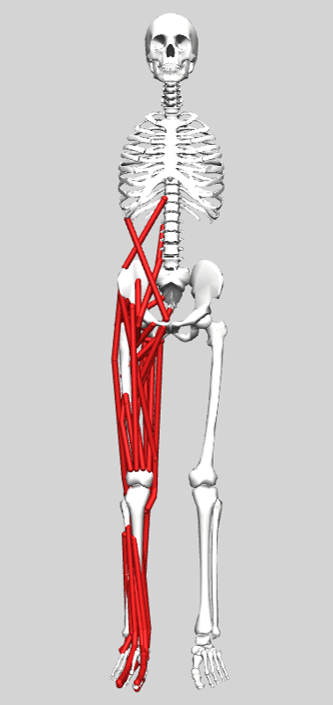
\includegraphics[width=0.3\textwidth]{Images/FullGait2392edit.png}
    }
    \hfill
    \subfloat[\label{monoMuscle}]{%
      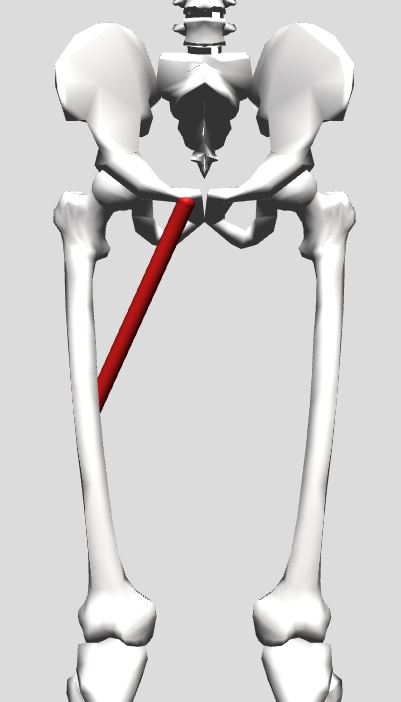
\includegraphics[width=0.3\textwidth]{Images/monoarticularMuscle.JPG}
    }
    \hfill
    \subfloat[ \label{biMuscle}]{
        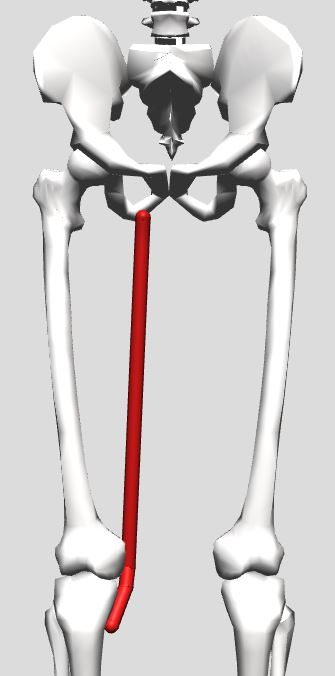
\includegraphics[width=0.3\textwidth]{Images/biarticularMuscle.JPG}
    }     
    \caption{(a) Full set of muscles for the right leg. (b) An example of a monoarticular muscle in OpenSim. (c) An example of a biarticular muscles in OpenSim.}
    \label{musclesOpenSim}
\end{figure}

\subsection{Moment Arm Calculation for Biarticulate Muscles}
Biarticular muscles are muscles in which they pass over two joints. This makes the problem difficult for two reasons. The first is that there are now two moment arms that we need to consider: the moment arm about the first joint and the moment arm about the second joint. This in of itself doesn't complicate the math that was described in the previous sections, but is something to keep note of.

The second reason for the added complexity is that there are two cases for a biarticulate muscle that dictate how the moment arms are calculated. In the first case, there are three points that describe the muscle pathing, and each point is located in one of the coordinate frames for the joints. The origin of the muscle is located in the original frame. The second point is located in the frame of the first joint. The third point is located in the last joint frame. 

The other case that arises from biarticulate muscle is a muscle geometry, with at least two points, in which the second point lies in the last coordinate frame. 

Passing over two joints results in the use of two transformation matrices. With biarticular muscles, there are two cases for their wrapping points. To illustrate the cases, consider a muscle, spanning the pelvis and knee, with three points: one attachment point, one wrapping point, and one insertion points.

The first case has all three points in their separate joint reference frames. The attachment point exists in the hip frame, the wrapping point exists in the femur frame, and the third point exists in the tibia frame. Because the next point in the series of muscle points will always exist in the next frame of reference, when calculating the moment arm, a point will only ever need to be multiplied by one transformation matrix.

The second case has the wrapping point and the insertion point in the tibia reference frame. This means that from the attachment point to the wrapping point, there are two transformation matrices between them. In order to calculate the moment arm about the knee, the attachment point will have to be shifted over by two transformation matrix. This does not give any information about the moment arm about the pelvis however. In order to calculate the moment arm about the pelvis, the attachment point and the wrapping point will have to be brought to the femur reference frame.
2 cases, one in which there is in an attachment point in each frame, one in which the attachment point is two frames over.

\subsection{Matlab Data Collation}

\section{Results}


\section{Discussion and Conclusion}


%Running concurrently with those next steps would be to begin implementing the muscle placements on a physical robot. 
%Useful as a platform for testing central pattern generator hypotheses

%Integrate a vestibular system and balance controller (reference wade and myself/other vestibular systems)
%Need to better measurements for larger diameter festo muscles
%Need to create a controller for achieving intermediate torques from the muscles, as opposed to assuming maximum torque at every position
%Interested in investigating the use of biarticulate muscles. 
%Currently only optimizing the point location for the attachment points that span a joint. Next want to look at moving via points as well as optimizing the number of via points needed. 

% ---- Bibliography ----
%
% BibTeX users should specify bibliography style 'splncs04'.
% References will then be sorted and formatted in the correct style.
%
\bibliographystyle{splncs03}

\bibliography{LMRef}

\end{document}
